\documentclass[12pt]{extarticle}
%Some packages I commonly use.
\usepackage[english]{babel}
\usepackage{graphicx}
\usepackage{framed}
\usepackage[normalem]{ulem}
\usepackage{amsmath}
\usepackage{amsthm}
\usepackage{amssymb}
\usepackage{amsfonts}
\usepackage{enumerate}
\usepackage[utf8]{inputenc}
\usepackage{float}
\usepackage[top=1 in,bottom=1in, left=1 in, right=1 in]{geometry}

%A bunch of definitions that make my life easier
\newcommand{\matlab}{{\sc Matlab} }
\newcommand{\cvec}[1]{{\mathbf #1}}
\newcommand{\rvec}[1]{\vec{\mathbf #1}}
\newcommand{\ihat}{\hat{\textbf{\i}}}
\newcommand{\jhat}{\hat{\textbf{\j}}}
\newcommand{\khat}{\hat{\textbf{k}}}
\newcommand{\minor}{{\rm minor}}
\newcommand{\trace}{{\rm trace}}
\newcommand{\spn}{{\rm Span}}
\newcommand{\rem}{{\rm rem}}
\newcommand{\ran}{{\rm range}}
\newcommand{\range}{{\rm range}}
\newcommand{\mdiv}{{\rm div}}
\newcommand{\proj}{{\rm proj}}
\newcommand{\R}{\mathbb{R}}
\newcommand{\N}{\mathbb{N}}
\newcommand{\Q}{\mathbb{Q}}
\newcommand{\Z}{\mathbb{Z}}
\newcommand{\<}{\langle}
\renewcommand{\>}{\rangle}
\renewcommand{\emptyset}{\varnothing}
\newcommand{\attn}[1]{\textbf{#1}}
\theoremstyle{definition}
\newtheorem{theorem}{Theorem}
\newtheorem{corollary}{Corollary}
\newtheorem*{definition}{Definition}
\newtheorem*{example}{Example}
\newtheorem*{note}{Note}
\newtheorem{exercise}{Exercise}
\newcommand{\bproof}{\bigskip {\bf Proof. }}
\newcommand{\eproof}{\hfill\qedsymbol}
\newcommand{\Disp}{\displaystyle}
\newcommand{\qe}{\hfill\(\bigtriangledown\)}
\setlength{\columnseprule}{1 pt}

\usepackage{hyperref}

\title{\textbf{SOCRaTEs}\\
\textbf{S}imulink \textbf{O}racles for \textbf{C}PS \textbf{R}equiremen\textbf{T}s\\ with unc\textbf{E}rtainty}
\author{Menghi Claudio, Nejati Shiva,  Khouloud Gaaloul,  Lionel Briand}
%\date{January 2019}
\date{\vspace{-5ex}}

%\geometry{paperwidth=170mm, paperheight=16383pt, left=40pt, top=40pt, textwidth=280pt, marginparsep=20pt, marginparwidth=100pt, textheight=16263pt, footskip=40pt}

\begin{document}

\maketitle

\vspace{1cm}
\begin{itemize}
\item Section~Overview provides an overview on SOCRaTEs.
\item Section~Installation and Project Creation describes how to install SOCRaTEs and how to create your first SOCRaTEs project.
\item Section~Using SOCRaTEs describes how to use SOCRaTEs.
\item Finally Section~Tutorial provides a  tutorial that describes how to use SOCRaTEs on a set of simple examples.
\end{itemize}





\section{Overview}

\begin{figure}
\caption{An Overview on SOCRaTEs.}
  \centering
    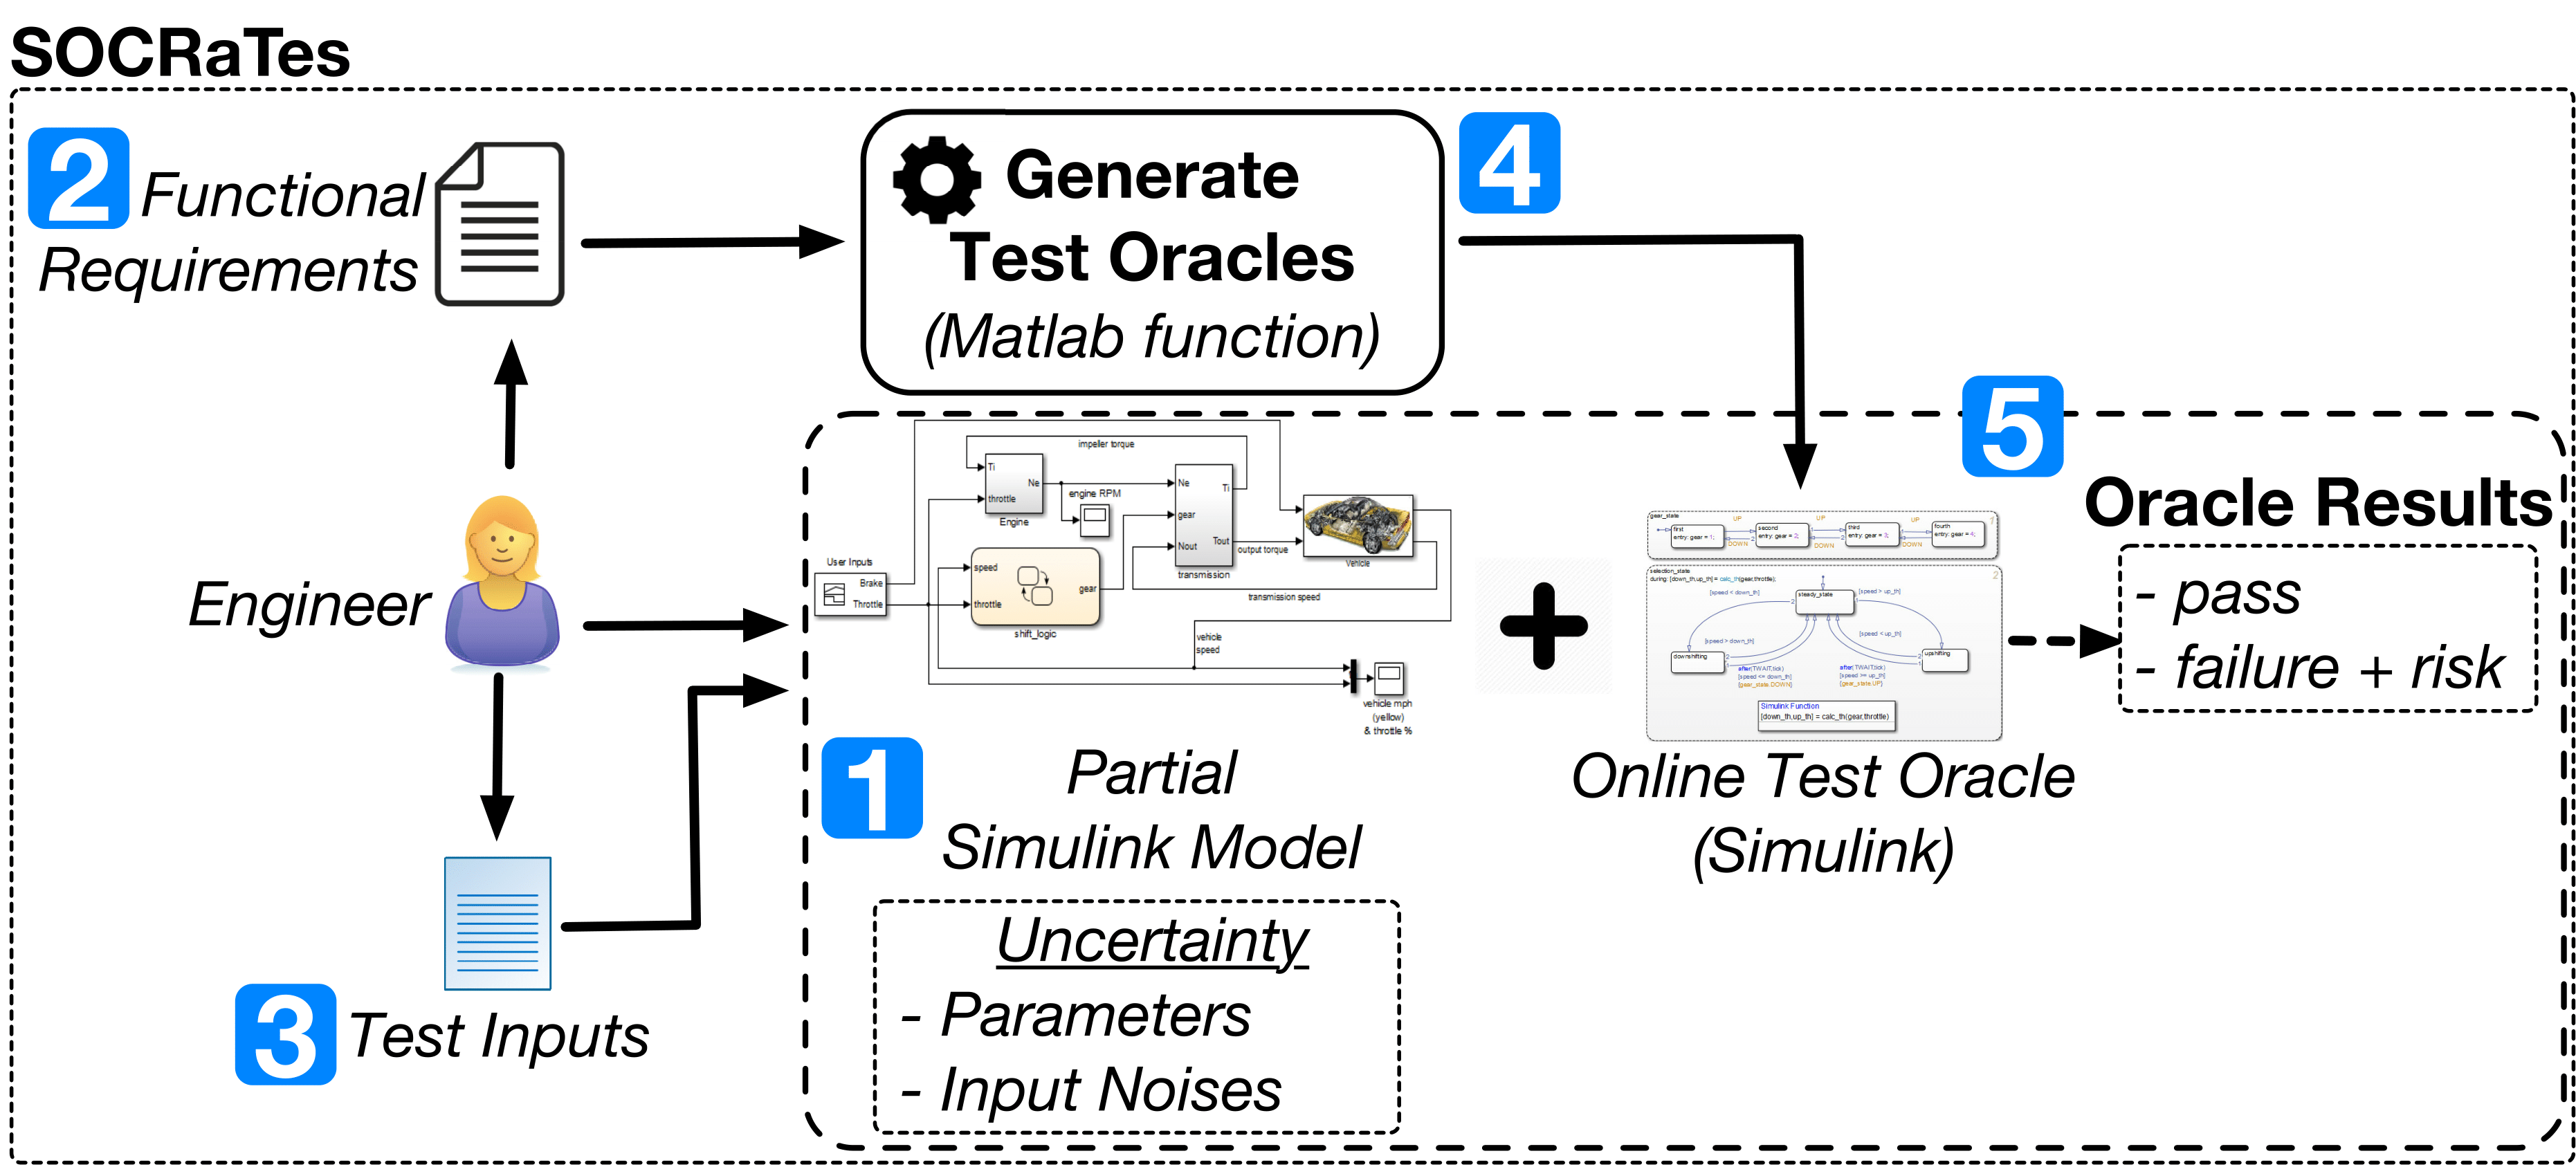
\includegraphics[width=0.7\textwidth]{Manual/Overview.pdf}
\end{figure}

\section{Installation and Project Creation}

\subsection{Prerequisite}
The following software must be installed on your laptop to run Socrates
\begin{itemize}
\item Eclipse (\url{https://www.eclipse.org/})
\item Java 1.8 or superior
\item Matlab/Simulink
\end{itemize}

\subsection{Installing Socrates}
Socrates can be installed by performing the following steps:
\begin{itemize}
\item Click on Help $>$ Install new Software $>$ Add $>$ Local
\item Select the Plugin folder;
\item Uncheck Group items by category;
\item Select Socrates SDK feature;
\item Click on Next $>$ Next $>$ I accept $>$ Finish.
\end{itemize}

\subsection{Creating a New Project}
To create a new project perform the following steps:
\begin{itemize}
\item File $>$ New $>$ Project;
\item Select Project from General;
\item Click on Finish;
\end{itemize}


\section{Using SOCRaTEs}

\subsection{Creating a your Requirements}
\begin{itemize}
\item Create a file .socrates (File $>$ New $>$ File);
\item When asked to convert into an Xtext project click on Yes.
\end{itemize}

\subsection{Generating the .m files using Socrates}
\begin{itemize}
\item copy the file demo.socrates within your workspace.
\item Change the file (e.g., add a new blank line) and save it
\item	When you save the file a file .m is automatically created in the folder src-gen/ModelName.
\end{itemize}

\subsection{Adding the oracles into your model}
\begin{itemize}
\item	Open the Simulink model test
\item	Copy the file Test\_Req.m into your workspace
\item	Run Test\_Req in Matlab
\item	tollerableriskTest\_Req=0;
\item	Run your simulation
\end{itemize}


\section{Tutorial}
We consider four different scenarios obtained by considering two different models and two requirements.

\subsection{The Considered Models}
The first model generates a sine wave with amplitude $2$ and frequency $1$ $rad/s$ that is represented in Figure~2.

\begin{figure}
\caption{The signal $e$ generated from the model Model 1.}
  \centering
    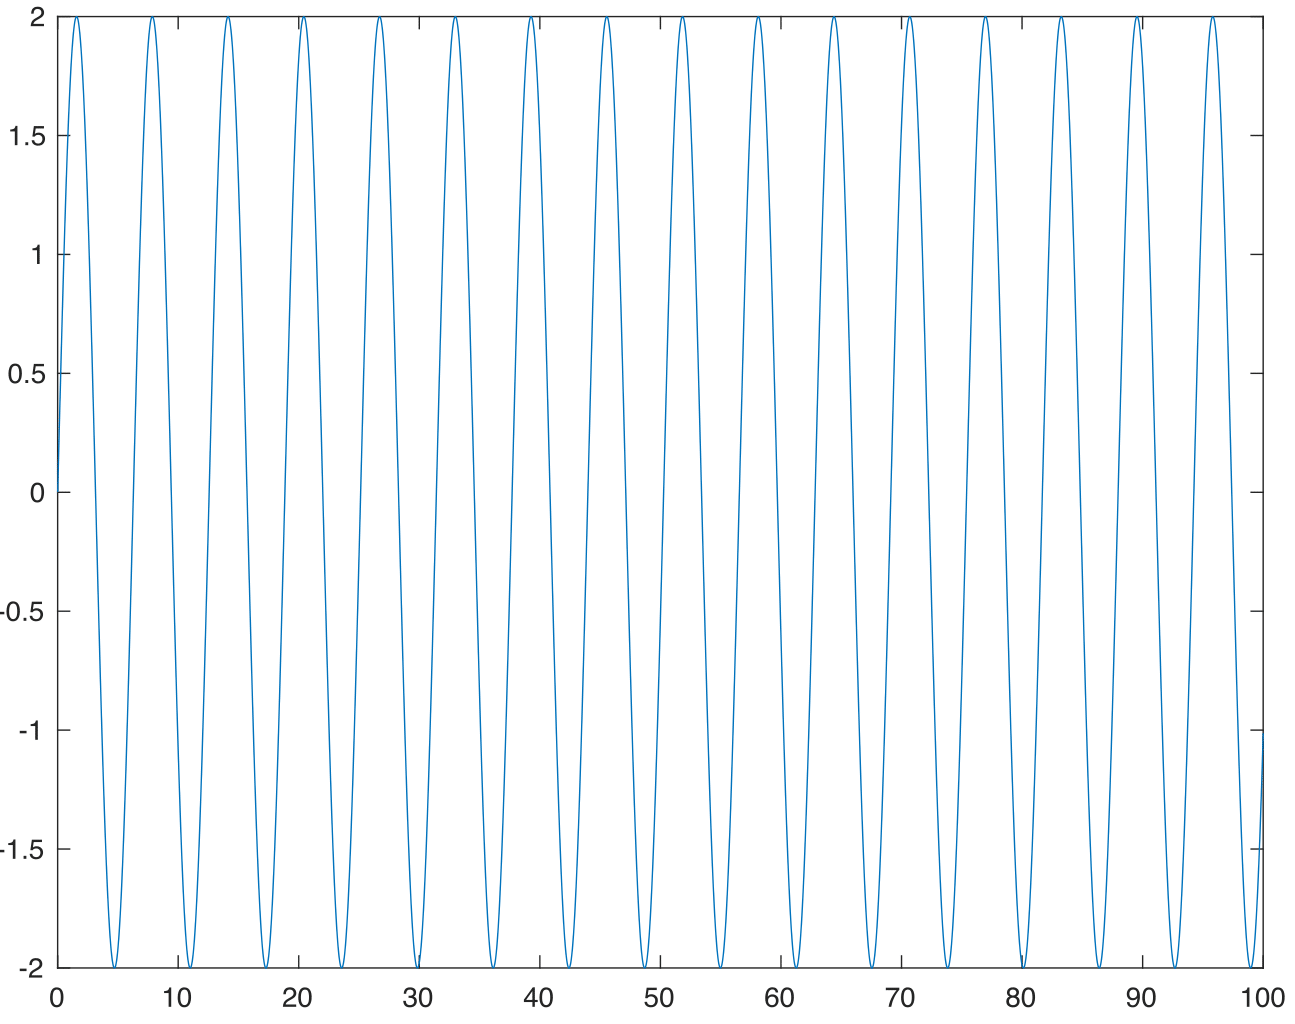
\includegraphics[width=0.5\textwidth]{Manual/Model1.pdf}
\end{figure}

The second model generates a sine wave with amplitude $0.5$ and frequency $1$ $rad/s$ that is represented in Figure~3.

\begin{figure}
\caption{The signal $e$ generated from the model Model 2.}
  \centering
    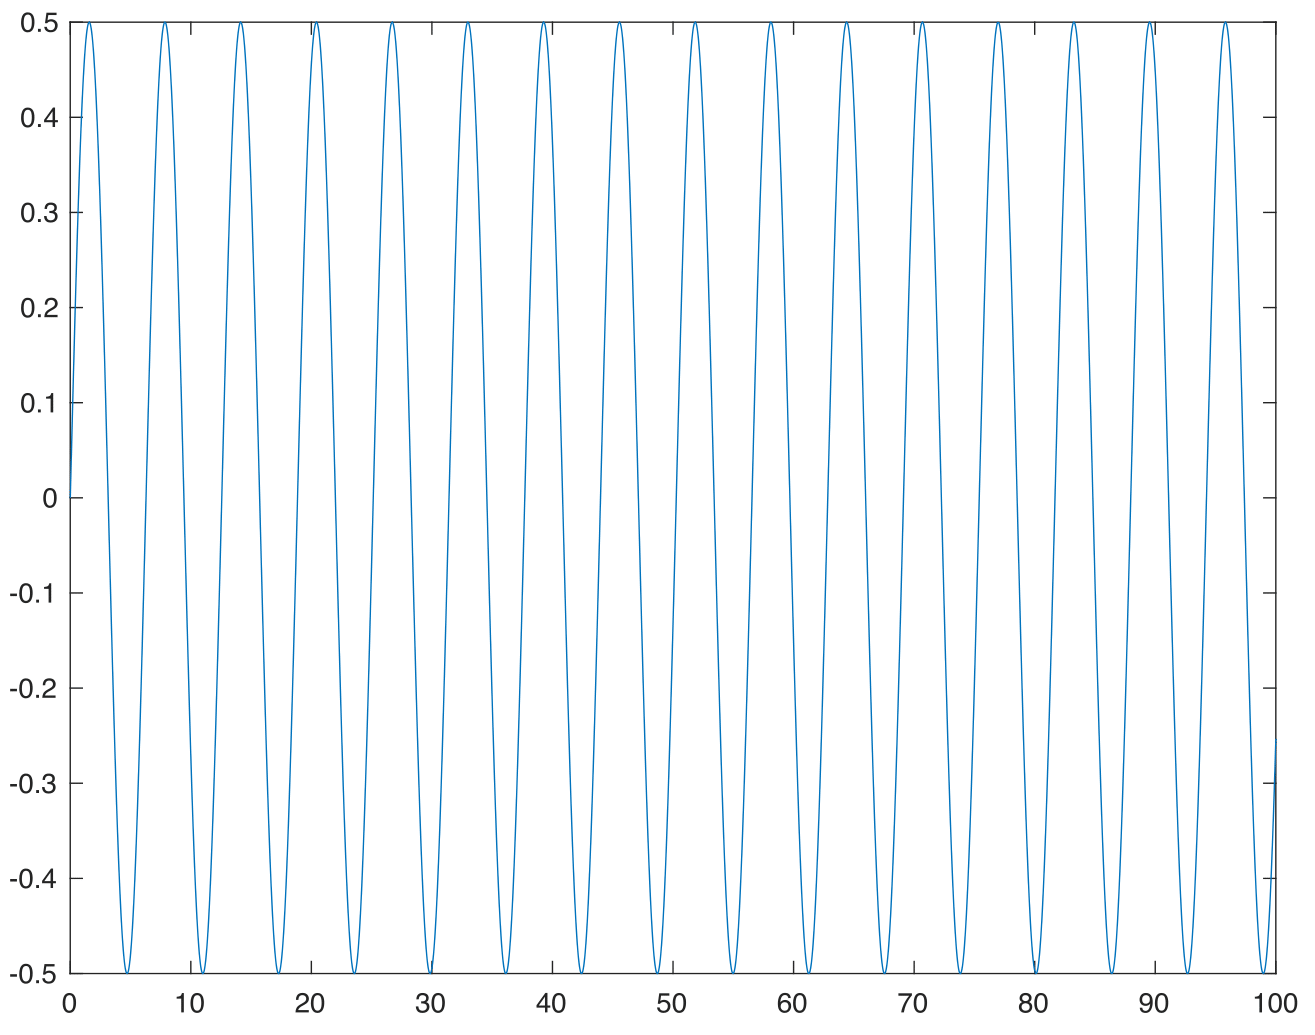
\includegraphics[width=0.5\textwidth]{Manual/Model2.pdf}
\end{figure}

\subsection{The Considered Requirements}



\section{Scenario 1}

The variable  $result\_Test\_Forall.Data$  contains the final result that for this simulation is: $-0.0109$.
Note that the result is negative. 
The property is indeed violated.

\section{Scenario 2}

The variable $result\_Test\_Forall.Data$ contains the final result that for this simulation is: $0.3333$.
Note that the result is positive.
The property is indeed satisfied.


\section{Scenario 3}

\section{Scenario 4}

\end{document}